\documentclass[a4paper]{article}
\usepackage[utf8x]{inputenc}
\usepackage[russian]{babel}
\usepackage[dvips]{graphicx}
%\usepackage{mathtext}
\usepackage{amsmath}
\usepackage{indentfirst}  % абзацный отступ после заголовка
\usepackage{misccorr}  % точка в заголовке
\usepackage{longtable}
\usepackage{verbatim}  % текст программы

\usepackage{setspace}  % интервалы
\onehalfspacing  % полутроный интервал

\usepackage{geometry}  % установка полей
\geometry{top=3.5cm,bottom=2cm,left=2cm,right=2cm}

\parindent=15mm
%\frenchspacing  % без пробелов после предложений

\usepackage{fancyhdr}  % колонтитулы
\pagestyle{fancy}  % смена стиля оформления страниц
\fancyhf{}  % очистка текущих значений
%\fancyhead[C]{\thepage}  % верхний колонтитул
\fancyhead[C]{\fontsize{14pt}{18pt}\selectfont\thepage}  % верхний колонтитул 
\renewcommand{\headrulewidth}{0pt}  % убрать разделительную линию

\relpenalty=10000  % запрещаем переносы формул

%\renewcommand{\rmdefault}{ftm}

\begin{document}
\begin{titlepage}
\begin{center}

\fontsize{14pt}{18pt}
\selectfont

\vfill
Федеральное агентство по образованию РФ\\
Новгородский государственный университет им.~Ярослава~Мудрого

\hrulefill

Кафедра ИТИС

\vfill
\vfill

{
\huge
Реализация алгоритмов поиска корней~уравнений\linebreak
методом половинного деления и методом хорд
}

\vfill

{
\begin{flushright}
Выполнил студент группы 9311\\
Лопатин А.С.
\end{flushright}
}

\vfill

Великий Новгород, 2009
\end{center}
\end{titlepage}

\setcounter{page}{2}  % продолжаем со 2-й страницы
\fontsize{14pt}{18pt}\selectfont

\section{Цель работы}
Реализовать алгоритмы поиска экстремума функции методами поразрядного
приближения и золотого сечения на языке программирования С++.

\section{Математическая модель решения}
Дана функция $f(x)$, границы $a$ и $b$, изначальное количество узлов оптимизации
$n$ и точность $\varepsilon$.
Необходимо найти экстремум функции между границами $a$ и $b$
с учетом точности $\varepsilon$.
Методы заключается в последовательном исключении частей отрезка.

Для метода поразрядного приближения выбирается шаг между узлами по формуле
$h=\frac{b-a}{n}$.
Начальное значение $x_1$ устанавливается в $a$, $x_2$ будет равным $x_1+h$,
т.~е. на шаг дальше.
Вычисляется 2 значения функции: $f_1=f(x_1)$ и $f_2=f(x_2)$.
Если $f_1<f_2$ (при поиске максимума; для минимума будет наоборот: $f_1>f_2$)
--- экстремум еще не пропустили, поэтому увеличиваем $x_1$ на шаг $h$.
Для определения чего мы ищем (минимум или максимум), можно умножить стороны
неравенства на $c$, принимающего значения $\{-1,1\}$, где --1 означает что мы
ищем минимум, а 1 --- максимум.
Тут же можно убедиться что экстремум присутствует в заданном
промежутке исходя из неравенства $x_1\le b$.
Если же мы пропустили экстремум --- отбрасываем отрезок $(x_2,b)$,
а $a$ теперь будет равен $x_2-2\cdot h$.
Новый шаг определяется по формуле $h=\frac{h}{n}$, а начальное значение $x$
снова задается на $a$.
Точность можно определять исходя из неравенства $|f_1-f_2|\le \varepsilon$.
Оптимальная точка~$x_{opt}$ выбирается средним арифметическим $a$ и $b$.

Метод золотого сечения заключается в делении отрезка в пропорциях
золотого сечения, которые определены следующим образом:
$$
\varphi=
\frac{\sqrt{5}+1}{2}\approx
1{,}6180339887=
\frac{b-a}{b-x_1}=
\frac{b-a}{x_2-a}
$$
где $\varphi$ --- пропорция золотого сечения,
$x_1$ и $x_2$ --- точки, которые делят отрезок $(a,b)$
на отрезки $(a,x_2)$ и $(x_1,b)$ в отношении золотого сечения.
Отсюда можно выразить значения этих точек: 
$x_1=b-\frac{(b-a)}{\varphi}$ и $x_2=a+\frac{(b-a)}{\varphi}$.
Тот из концов отрезка, к которому среди новых точек ближе оказалась та,
значение в которой минимально (при поиске максимума; для минимума ---
наоборот) отбрасывают.
Точность можно определять исходя из исходя из неравенства $|b-a|\le\varepsilon$.
Оптимальная точка опять же определяется средним арифметическим
точек $x_1$ и $x_2$ (или $a$ и $b$).

\section{Спецификация}
Таблица переменных:
{
\fontsize{10pt}{12pt}\selectfont
\begin{longtable}{|p{1.5cm}|l|p{2.5cm}|l|p{2cm}|p{4.5cm}|}
\hline
Исходное значение & Идентификатор & Тип & Вид & Размерность & Назначение\\
\hline
$\varphi$ & FI & Вещественная константа & Простой & -- &
Пропорция золотого сечения\\
\hline
$a$ & a & Вещественный & Простой & -- & Левая граница\\
\hline
$b$ & b & Вещественный & Простой & -- & Правая граница\\
\hline
$\varepsilon$ & eps & Вещественный & Простой & -- & Точность\\
\hline
$n$ & n & Целый & Простой & -- & Количество узлов оптимизации\\
\hline
func & func & Целый & Простой & -- & Номер функции\\
\hline
maxima & maxima & Логический & Простой & -- & Вид экстремума\\
\hline
$c$ & c & Целый & Простой & -- & Множитель для поиска минимума или максимума\\
\hline
$i$ & i & Целый & Простой & -- & Счетчик итераций\\
\hline
$h$ & h & Вещественный & Простой & -- & Шаг между узлами оптимизации\\
\hline
$x_1$ & x1 & Вещественный & Простой & -- & Аргумент функции\\
\hline
$x_2$ & x2 & Вещественный & Простой & -- & Аргумент функции\\
\hline
$f_1$ & f1 & Вещественный & Простой & -- & Значение функции\\
\hline
$f_2$ & f2 & Вещественный & Простой & -- & Значение функции\\
\hline
$x_{opt}$ & xopt & Вещественный & Простой & -- & Оптимальный аргумент функции\\
\hline
$y_{opt}$ & y & Вещественный & Простой & -- & Оптимальное значение функции\\
\hline
\end{longtable}
}

\newpage
\section{Алгоритм}

\subsection{Процедура <<bitwise\_approx>>}
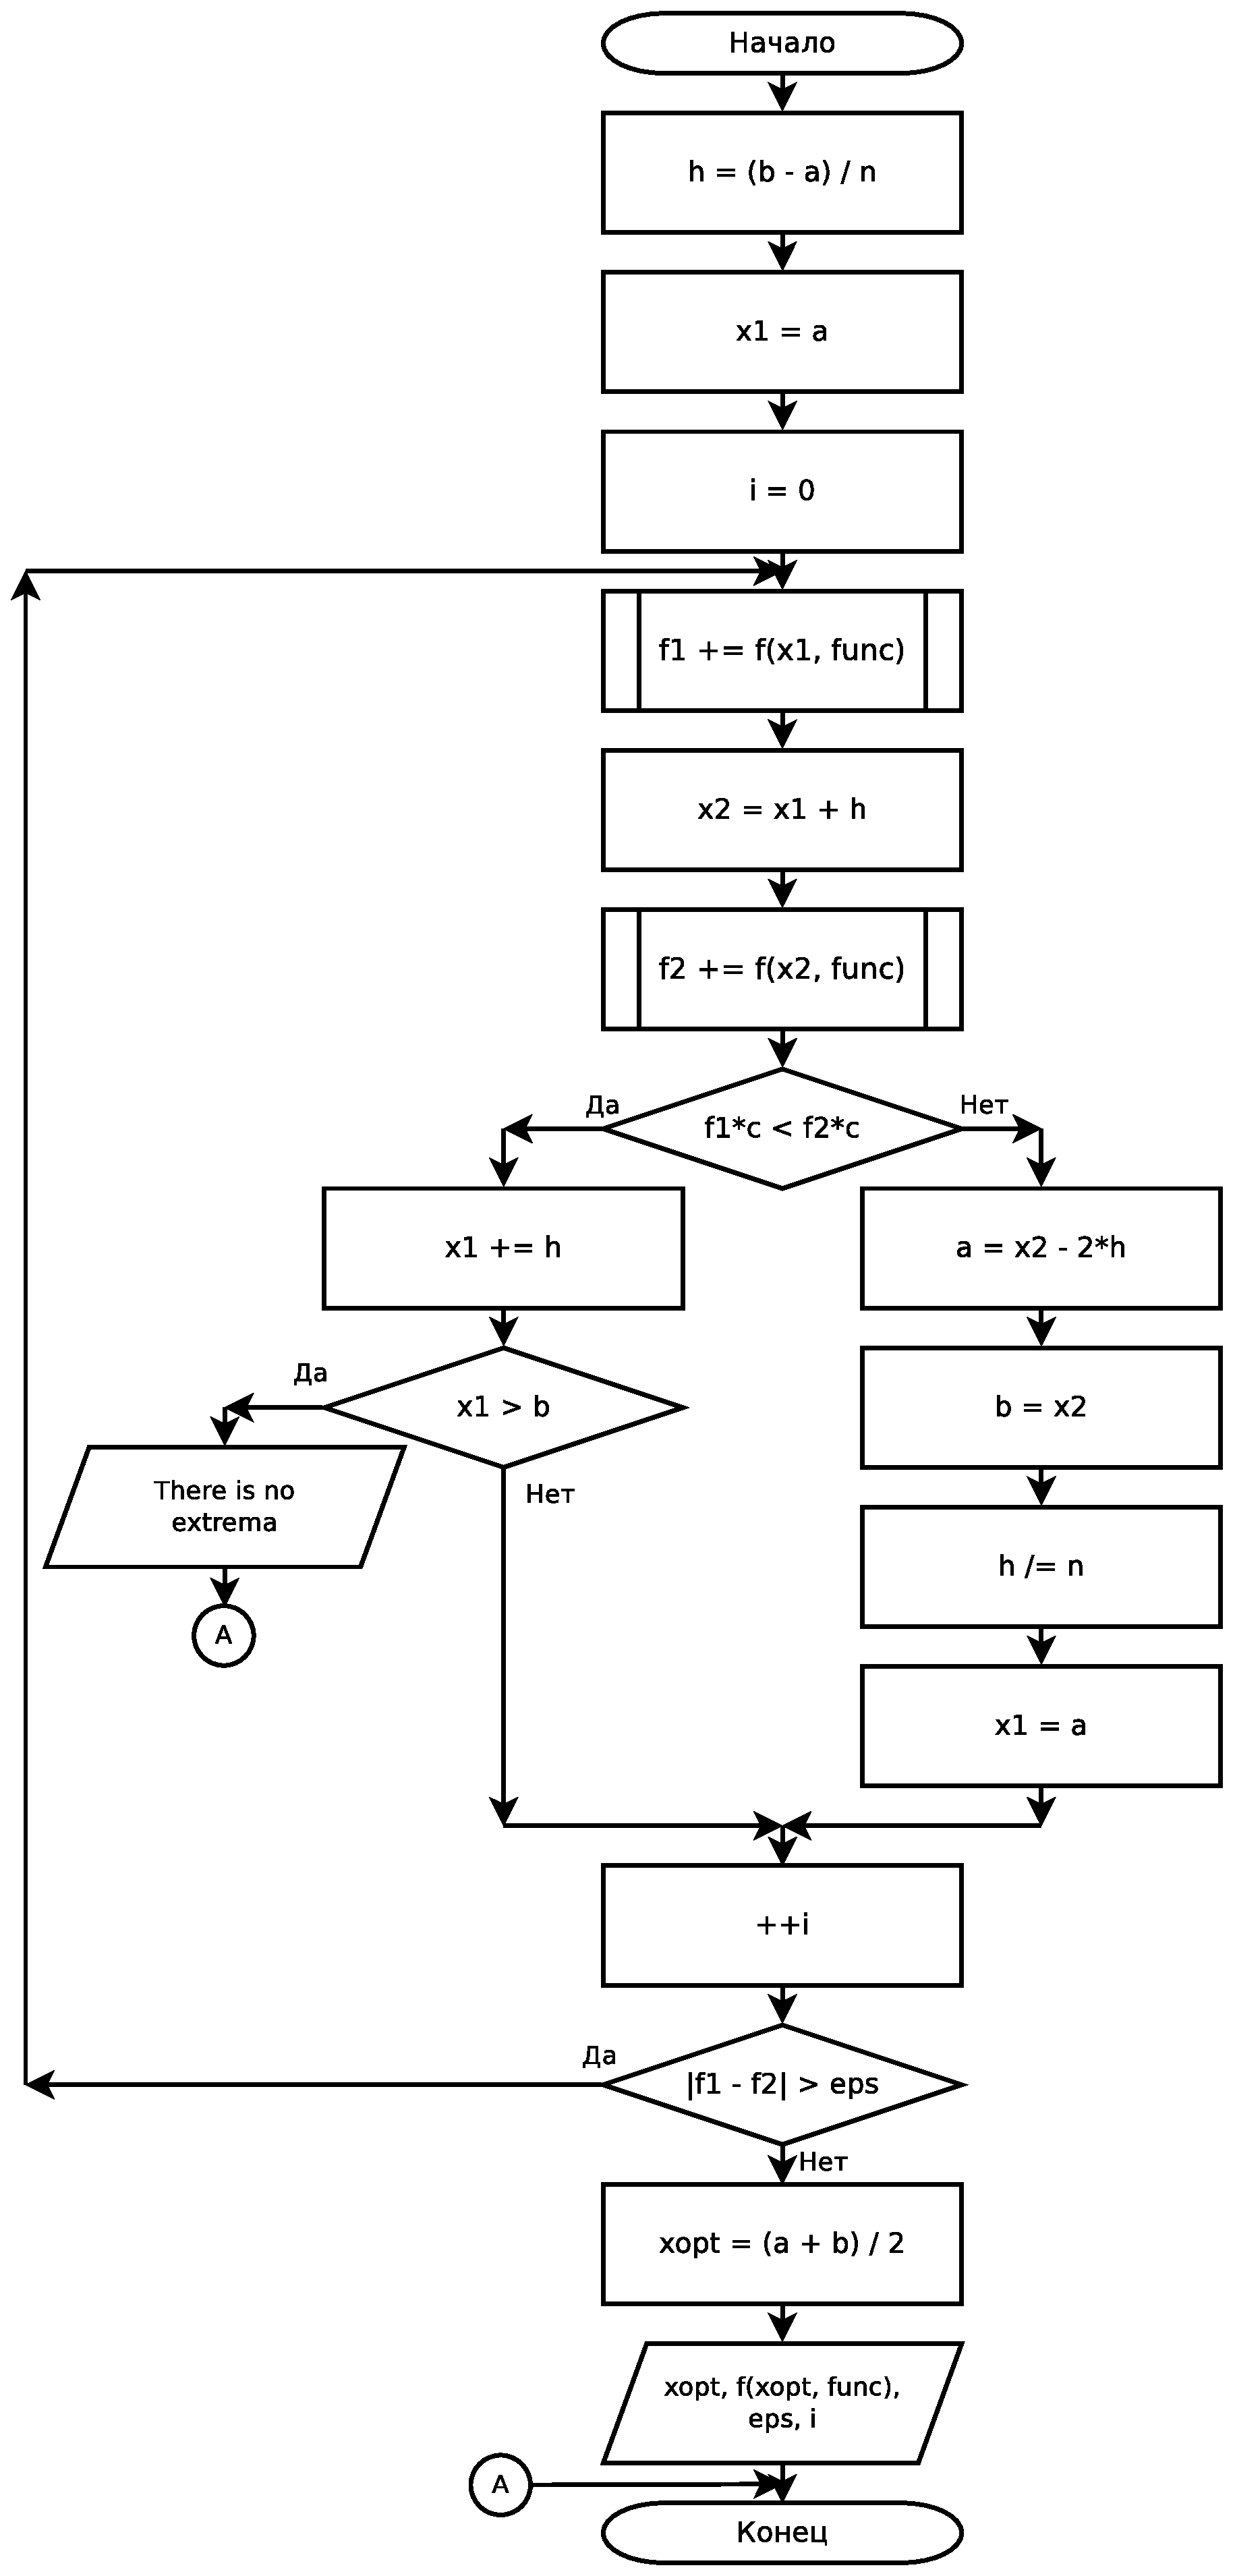
\includegraphics[scale=0.35]{schemes/bitwise_approx}

\subsection{Процедура <<golden\_section>>}
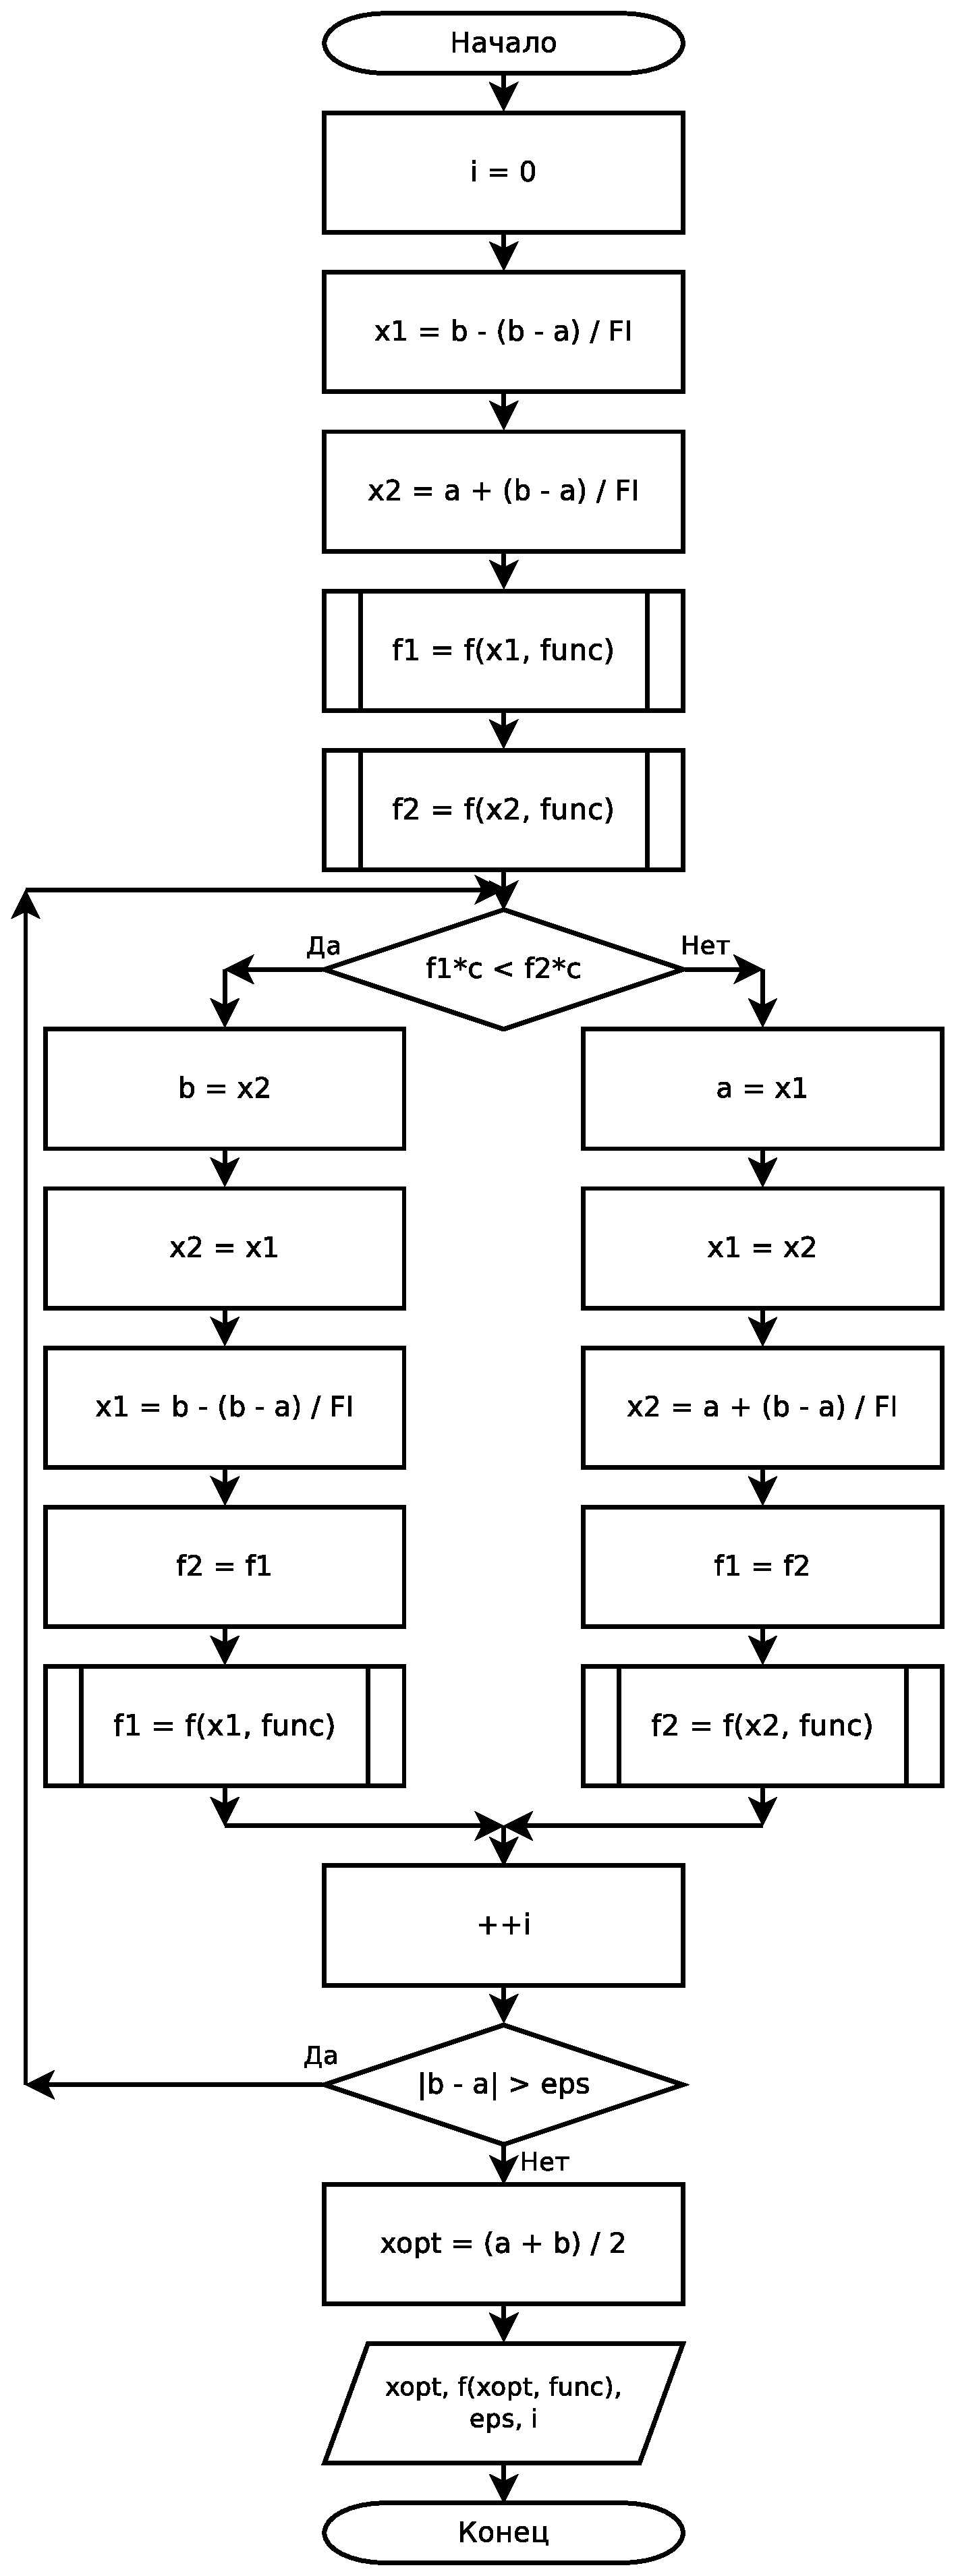
\includegraphics[scale=0.35]{schemes/golden_section}

\subsection{Функция <<$f(x)$>>}
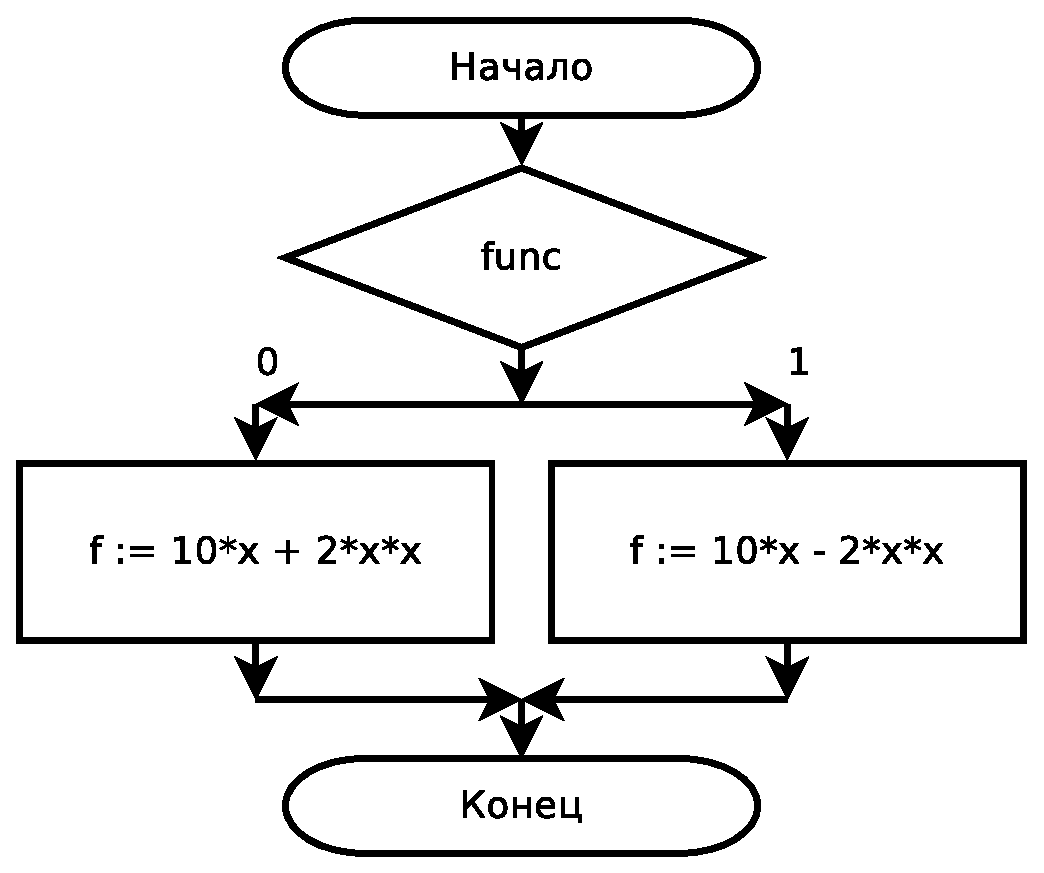
\includegraphics[scale=0.35]{schemes/f}

\subsection{Функция <<main>>}
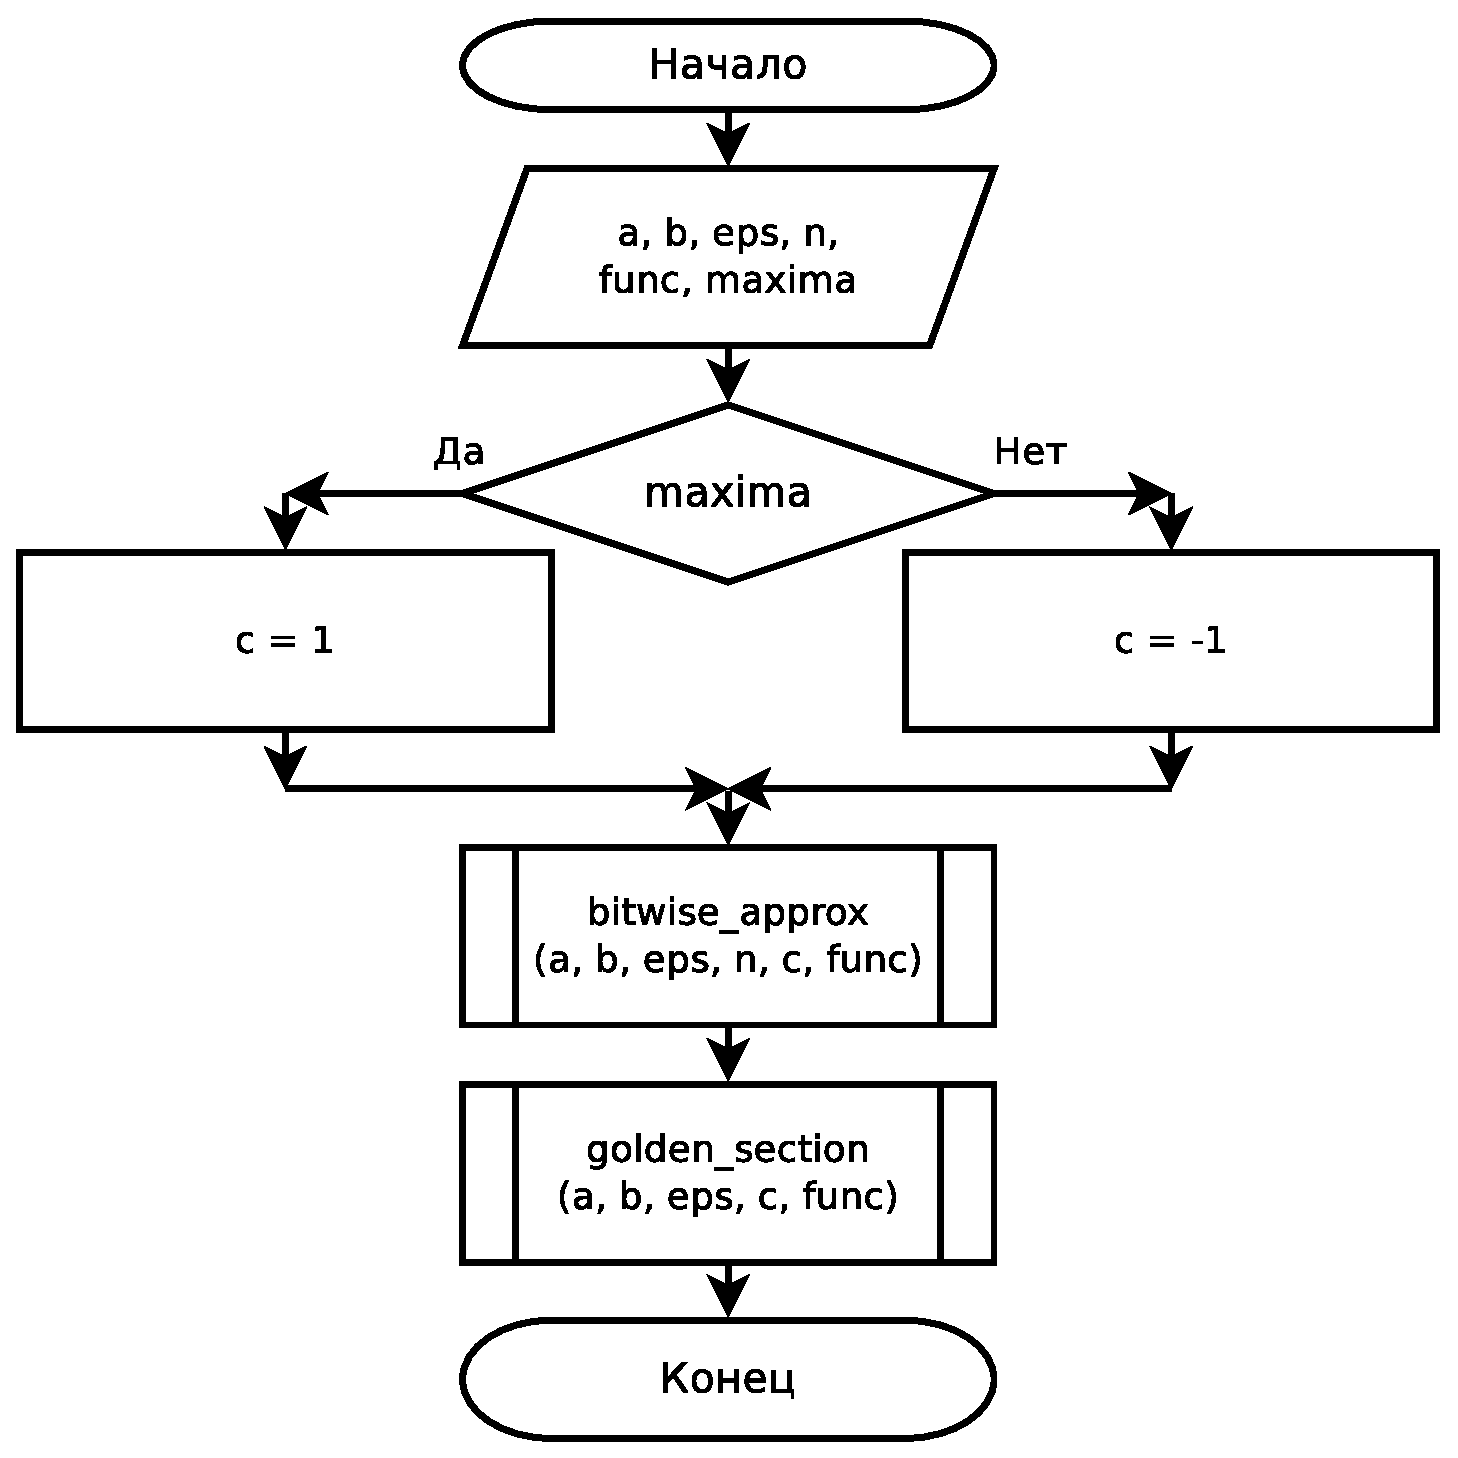
\includegraphics[scale=0.35]{schemes/main}

\section{Программа}
{
\fontsize{12pt}{14pt}
\selectfont
\verbatiminput{../4.cc}
}

\section{Шаблон ввода исходных данных}
{
\fontsize{12pt}{14pt}
\selectfont
\begin{verbatim}
-100
100
0.0001
400
0
0
\end{verbatim}
}

\section{Шаблон вывода результата}
{
\fontsize{12pt}{14pt}
\selectfont
\begin{verbatim}
Bitwise approximation: xopt = -2.5, f(xopt) = -12.5, eps = 0.0001, i = 581
Golden section method: xopt = -2.50001, f(xopt) = -12.5, eps = 0.0001, i = 31
\end{verbatim}
}

\section{Вывод}
Исходя из проделанной работы можно сделать вывод, что метод золотого сечения
превосходит по сходимости метод поразрядного приближения.

\end{document}
